\documentclass[conference]{IEEEtran}
\usepackage[english]{babel}
\usepackage[autostyle]{csquotes}
\usepackage{amsmath,amssymb,amsfonts}
\usepackage{algorithmic}
\usepackage{graphicx}
\graphicspath{{images/}}
\usepackage{textcomp}
\usepackage{xcolor}
\usepackage[outputdir=output]{minted}
%\usemintedstyle{autumn} % friendly, colorful
%\newminted{c}{mathescape, linenos, numbersep=5pt, gobble=0, frame=lines, framesep=2mm}
%\definecolor{background}{gray}{0.90}
%\newminted{bash}{bgcolor=background}
%\newminted{console}{bgcolor=background}
%\usemintedstyle[console]{bw}
\def\BibTeX{{\rm B\kern-.05em{\sc i\kern-.025em b}\kern-.08em
    T\kern-.1667em\lower.7ex\hbox{E}\kern-.125emX}}
\pdfinfo{
/Title (Semantics Generation For A 3D Environment Using Ray Tracing and RenderMan)
/Author (Mark Wesley Harris)
}
\begin{document}

\title{Semantics Generation For A 3D Environment Using Ray Tracing and RenderMan}

\author{\IEEEauthorblockN{Mark Wesley Harris}
\IEEEauthorblockA{\textit{CS5800 Computer Graphics, Fall 2019} \\
\textit{University of Colorado Colorado Springs}\\
Colorado Springs, United States \\
wharris2@uccs.edu}}

\maketitle

\begin{abstract}
Here is proposed a study of scene semantics
using ray tracing and current rendering techologies.
It is important to understand the relationship between
a given object in a 3D environment and what is rendered to
the screen.
This research will be applied to a broader machine learning
architecture for dynamically generating frames
given scene and render data.
\end{abstract}

\section{Introduction}
\label{sec:introduction}
Access to good training data is necessary
in order to harness the power of machine learning.
One such data to be studied is the relationship
between a 3D environment and the
rendered frame(s) it produces.
For the purposes of this document, this relationship is
referred to as the semantics of the given 3D scene --
i.e. the description of the 3D environment and its complexity
in relation to what is rendered.
This study is key to understanding and perhaps improving the
render pipeline and current rendering techologies.
However, extracting this data from the render process into a usable
format is not straightforward.

In this document is proposed a study of scene semantics and the development of a
usable algorithm to generate relevant semantic data from 3D environments.
We will focus on generating these semantics and study
how they may influence developments of
machine learning models in Computer Graphics.

\section{Related Work}
\label{sec:related_work}
\subsection{Ray Tracing}
Ray tracing is the study of how light behaves in a given environment.
Figure \ref{fig:raytrace}
shows a ray tracing problem studied in 1986, where light rays were mapped from
the viewer to a light source. Avro \textit{et al.}
discuss the difficulty of this problem,
as it involves taking into consideration material properties, light sources,
and where the viewer is looking \cite{backwards_raytrace}.

\begin{figure}[htbp]
\centerline{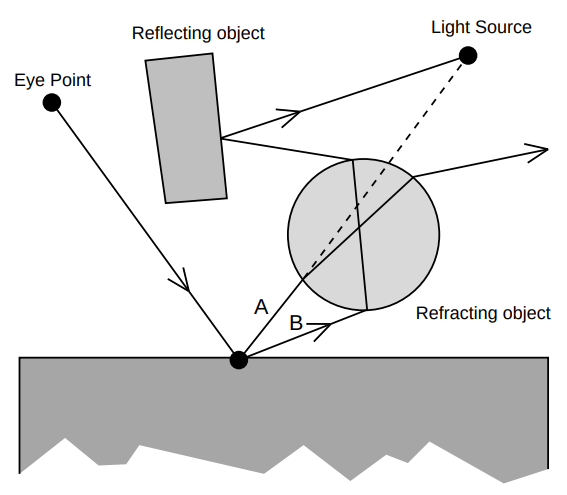
\includegraphics[width=5cm]{raytrace.png}}
\caption{Example of a problem in ray tracing \cite{backwards_raytrace}.}
\label{fig:raytrace}
\end{figure}

Technological advancements since 1986 have greatly improved ray tracing capabilities.
The ray tracing basics described by Scratchapixel 
provides a walkthrough with code samples for casting rays from the camera
\cite{raytrace_walkthrough}.

\subsection{Rendering Technologies}
Two renderers that are now highly developed are the Arnold Renderer \cite{arnold}
and the RenderMan renderer \cite{renderman}. Each of these renderers
function differently.
RenderMan -- which is maintained by Pixar Animation Studios --
was chosen to be the renderer software for the purposes of this project,
since it is arguably the most advanced renderer developed to date.

The RenderMan Interface is proposed to be used as a gateway
into producing the bulk of scene semantics.
The RenderMan Interface provides implementations for rendering
``\dots hidden surfaces, spatial filtering, dithering, motion blur, depth of field,
flat and curved surfaces, objects, constructive solid geometry,
and programmable shading to express lighting conditions, shadows, and surface appearances,
with sophisticated control over color, texture, and reflectivity''
\cite{renderman_docs}.
Many of these attributes are out of scope
for this project, however they may later be explored in order to test the capabilities
of what is developed.

\subsection{Architectural Overview}
\label{subsec:architecture}
The work proposed here will be applied to a machine learning framework
based off of the architecture
developed by Ma \textit{et al.} \cite{pose_guided_image_generation}.
Their research showed that a 2-stage generator-discriminator system worked well for generating
and refining images from one pose to another.
See Figure \ref{fig:block_diagram} for a basic block diagram of the adapted architecture
proposed for this project.
The most important component to the architecture as a whole
is Generator I, which uses a combination of pixel and pose data to generate a
low resolution image containing global structures found in the
source data.

\begin{figure}[htbp]
\centerline{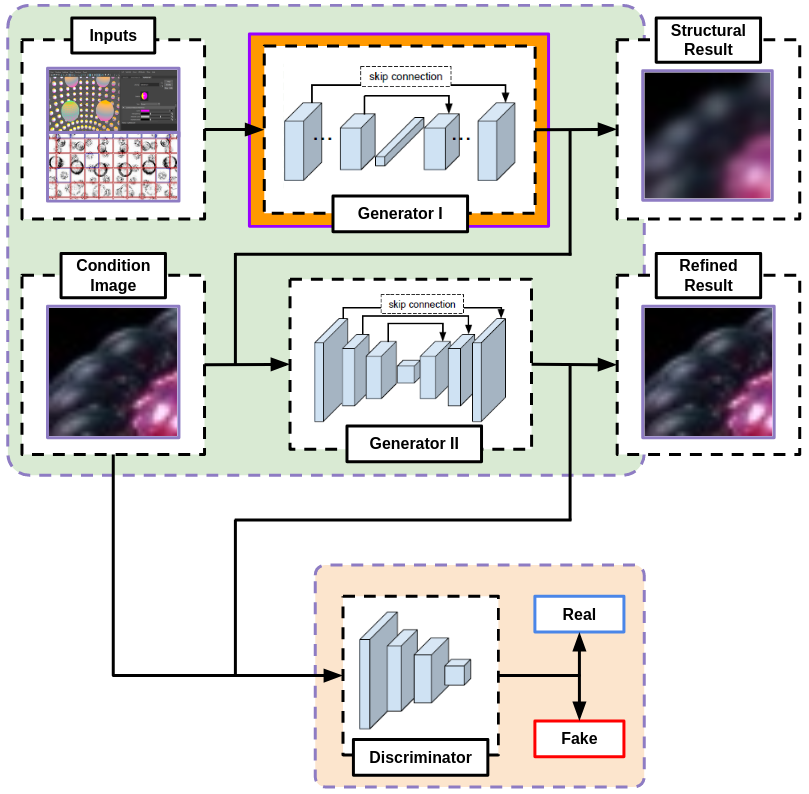
\includegraphics[width=8cm]{block_diagram.png}}
\caption{Block diagram for proposed architecture \cite{thesis_harris}.}
\label{fig:block_diagram}
\end{figure}

\section{Proposed Work}
\label{sec:proposed_work}
\subsection{Development and Expectations}
Most of the development for this project will be in RenderMan and Autodesk Maya,
with some pre/post-processing to occur intermittently in Python.
Published research papers, online tutorials, and other resources will be
utilized in order to develop a method for exporting semantic data from an Autodesk Maya scene
rendered with RenderMan.

\subsubsection{Autodesk Maya}
Autodesk Maya (Maya for short) is a 3D animation and modeling software that will be utilized
for creating the 3D animated scenes input into the render pipeline.
The scenes created will be of varying complexity to ensure that all aspects of a
render will be taken into account.
Scenes will involve dynamic camera movement, lighting, and material attributes, in order
to represent the complicated use-cases for this project.

Maya Embedded Language (MEL) or Python scripting
will be utilized within Maya in order to produce some semantic data, such as finding neighboring
objects and generating a heirarchical tree. Export functions (OBJ, FBX, etc.) will also be explored
as sources of further semantic data that can be preprocessed from within the software.
Figure \ref{fig:maya} shows an example of the GUI for Maya 2019 software.

\begin{figure}[htbp]
\centerline{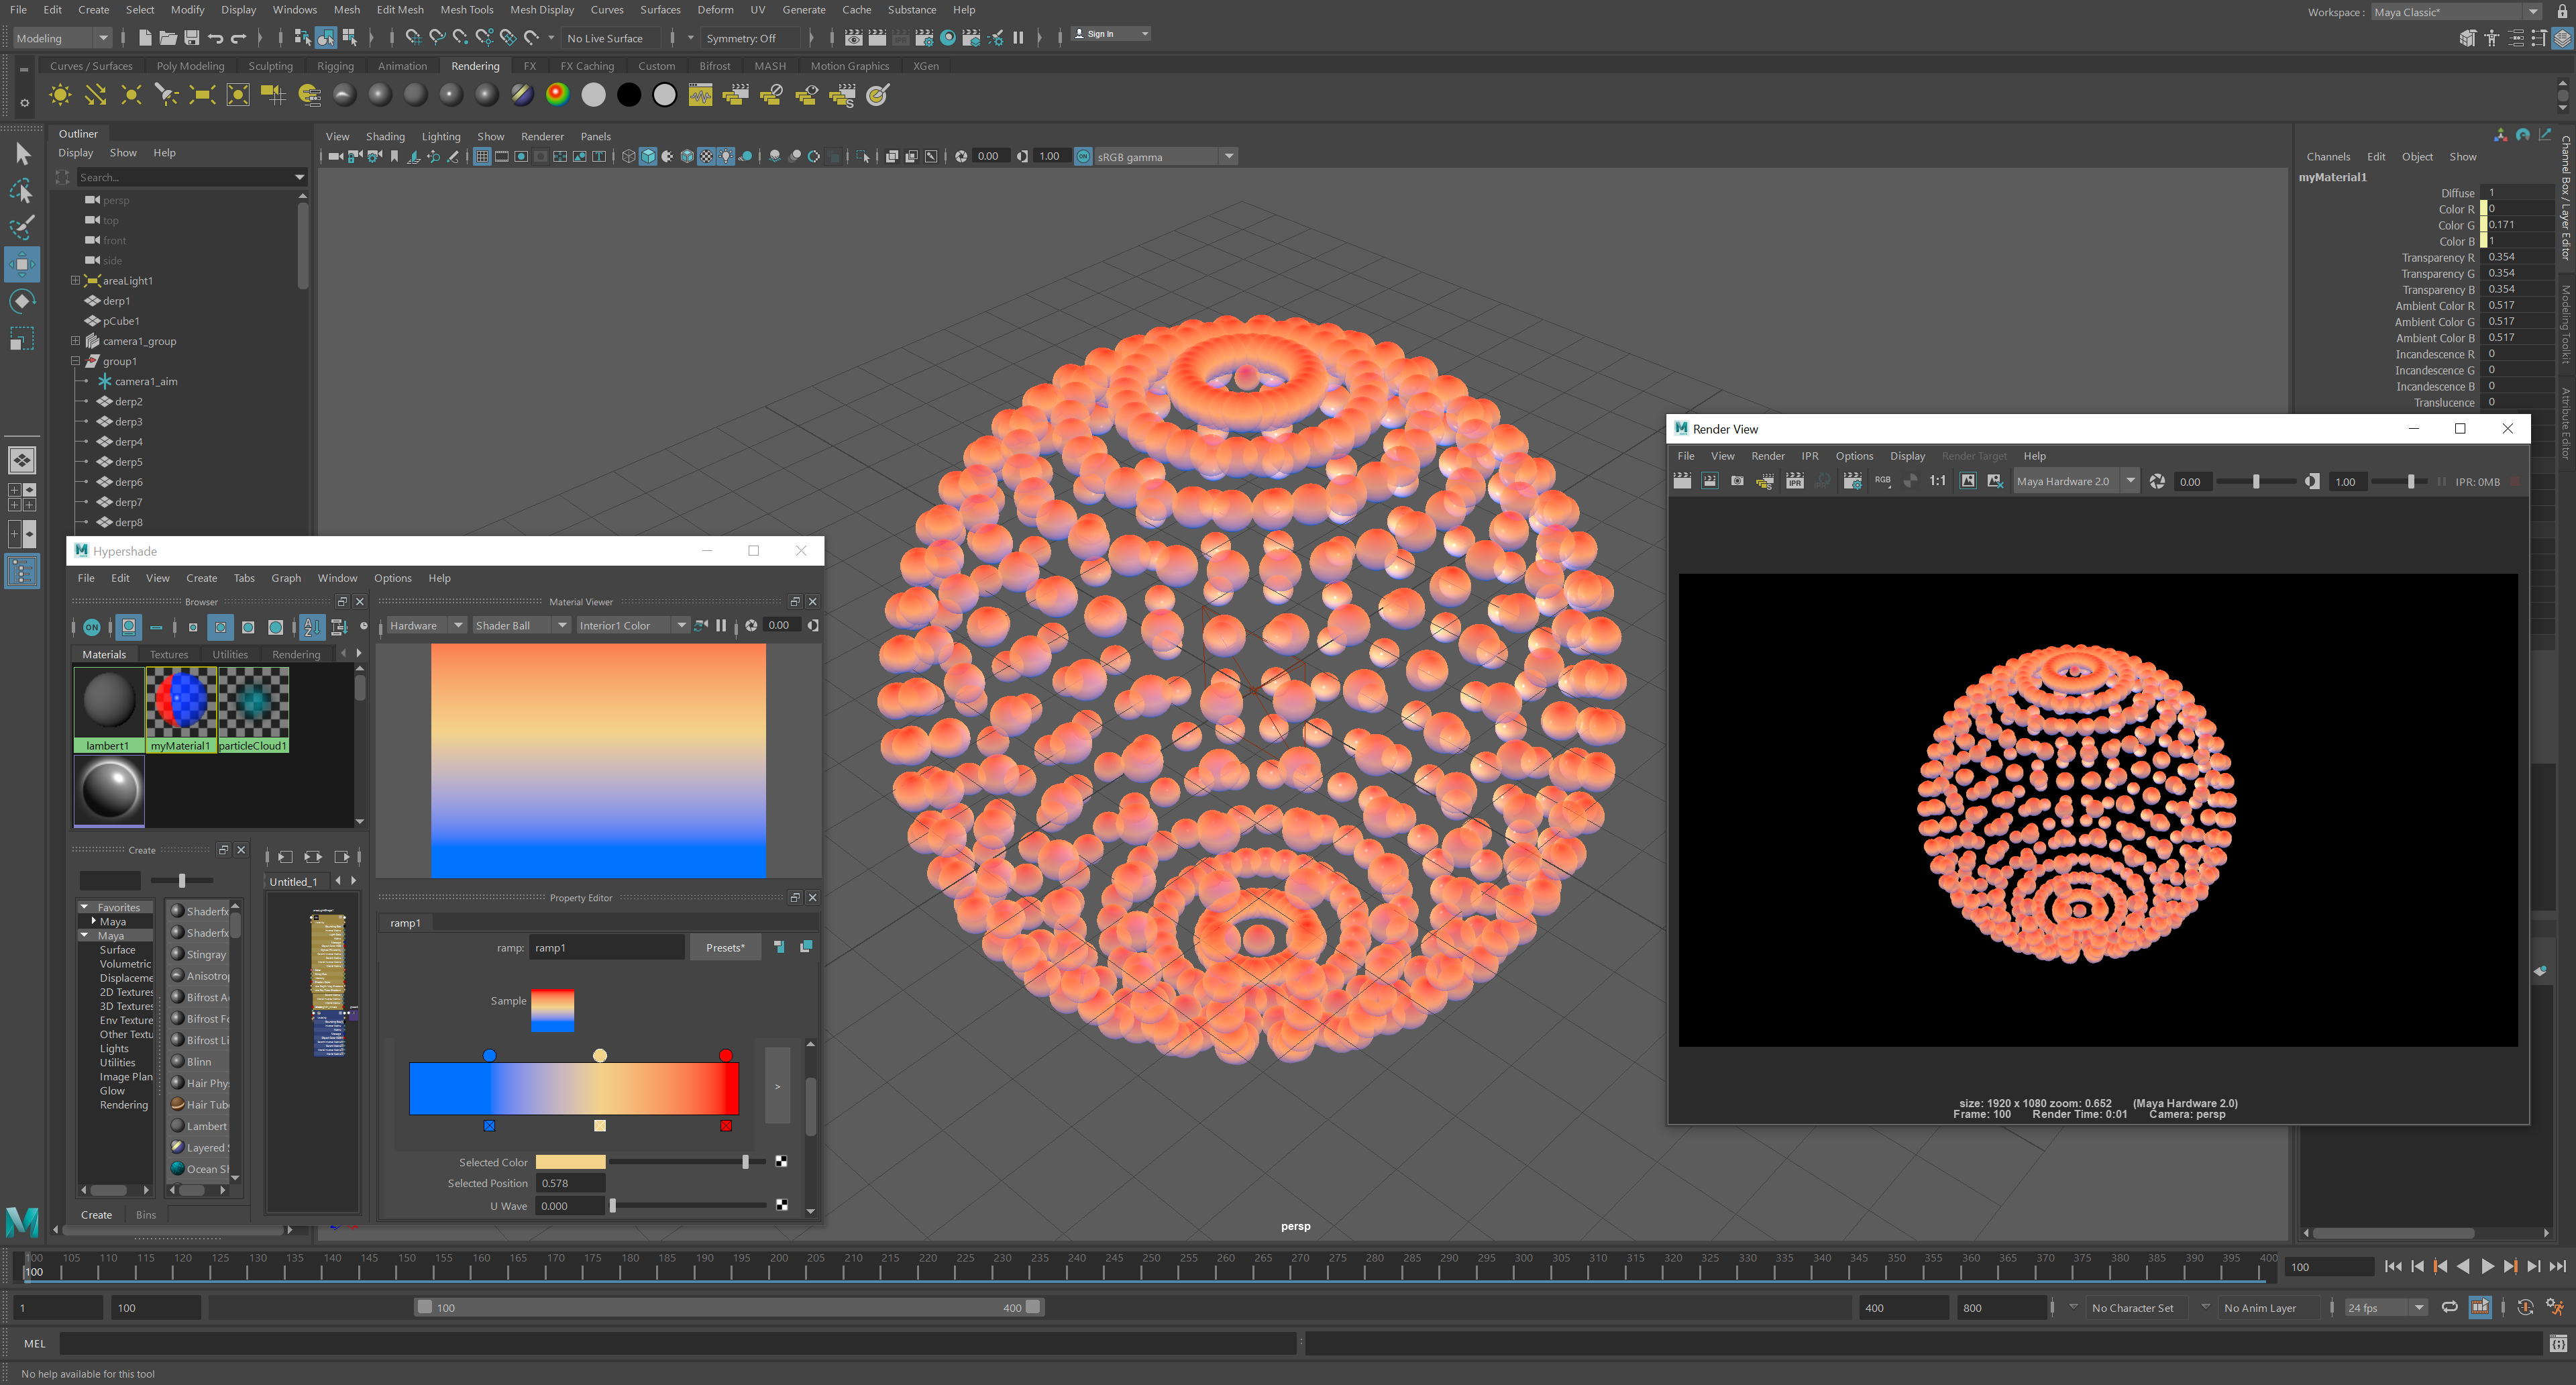
\includegraphics[width=8cm]{maya.png}}
\caption{Autodesk Maya workspace.}
\label{fig:maya}
\end{figure}

\subsubsection{RenderMan}
RenderMan will be used to build a render pipeline that will not only render advanced images
of 3D scenes, but also calculate and export scene semantics.
It is predicted that this will be possible through the use of raytracing or ray sampling.
The walkthrough comparison of OpenGL to RenderMan found in \cite{renderman_opengl}
may prove useful for development.
It is also expected that the RenderMan documentation found in \cite{renderman_docs}
will be referred to as well.
See Figure \ref{fig:renderman} for examples of dynamic scenes rendered with RenderMan.

\begin{figure}[htbp]
\centerline{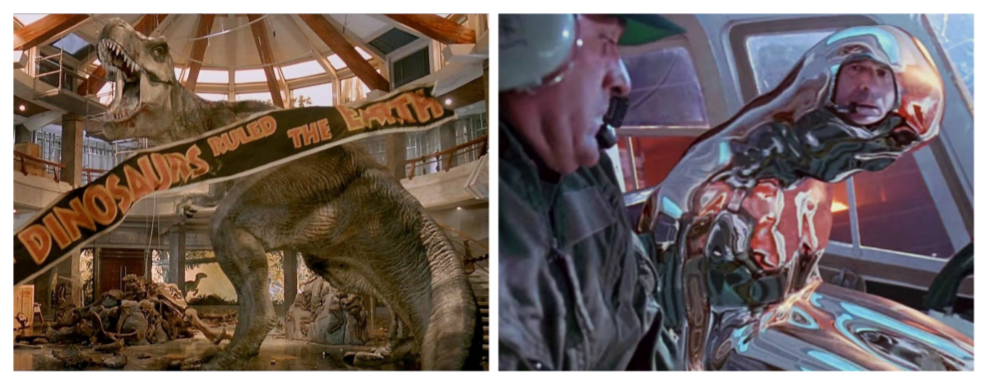
\includegraphics[width=8cm]{renderman.png}}
\caption{Path-traced images rendered with RenderMan \cite{renderman}.}
\label{fig:renderman}
\end{figure}

\section{Semester Timeline}
\label{subsec:semester_timeline}
\textbf{\textit{9/10 -- 9/17} Documentation for Proposal (1 week)}
\begin{itemize}
\item Research -- Collect research for ray tracing, RenderMan, and Autodesk Maya pipeline.
\end{itemize}
\textbf{\textit{9/17 -- 9/24} Environment Setup (1 week)}
\begin{itemize}
\item Fundamentals -- Build computer and setup environment.
\item Maya -- Setup a basic scene.
\item RenderMan -- Download and install.
\end{itemize}
\textbf{\textit{9/24 -- 10/3} Project 1 (1 and a half weeks)}
\begin{itemize}
\item Test Render Pipeline -- Create a dynamic export rendered in RenderMan for Project 1.
\end{itemize}
\textbf{\textit{10/3 -- 10/22} Explore RenderMan (3 weeks)}
\begin{itemize}
\item Research -- Further research and analysis into ray tracing in RenderMan.
\item Basic working pipeline -- Work from animation file used in \cite{thesis_harris}
to create a basic working pipeline.
\item Basic working script -- Use the RenderMan documentation \cite{renderman_docs}
to start working on scripts for the RenderMan Interface.
\end{itemize}
\textbf{\textit{10/22 -- 10/29} Midterms Wiggle Room (1 week)}\\
\textbf{\textit{10/29 -- 11/12} Ray Tracing (2 weeks)}
\begin{itemize}
\item Program ray tracing -- Use OpenGL to RenderMan discussion \cite{renderman_opengl}
and ray trace walkthrough \cite{raytrace_walkthrough} as references.
\end{itemize}
\textbf{\textit{11/12 -- 11/26} Export Object Semantics (2 weeks)}
\begin{itemize}
\item Generate Semantics -- Find semantic information associated with each pixel.
\item Export -- Save semantics in a parsable format for (optional) postprocessing.
\end{itemize}
\textbf{\textit{11/26 -- 12/3} Thanksgiving Break (1 week)}
\begin{itemize}
\item Complete Work -- Final completion of work.
\item Clean Up -- Code and repository clean up.
\end{itemize}
\textbf{\textit{12/3 -- 12/10} Documentation for Final Presentation (1 week)}
\begin{itemize}
\item Documentation -- Slides and other documentation.
\item 12/10 -- Last day to present.
\end{itemize}
\textbf{\textit{12/10 -- 12/17} Finals Wiggle Room (last week)}

\section{Conclusion}
\label{sec:conclusion}
We propose a study of the relationship between objects in a 3D scene and rendered images.
Semantics data is easily recognizable by humans, but much harder for machines.
Automating the process is a complicated task that will involve much consideration over
scene dynamics and the relationship of objects to what is rendered.
Ray tracing is also a concept
key to many difficult tasks, and this project is an
opportunity to explore the implementation of ray tracing and its application
to difficult problems in Computer Graphics.
Not only will the project benefit ongoing research \cite{thesis_harris},
but it will also stand as a separate body of work from which further research can sprout from.

\bibliographystyle{IEEEtran}
\bibliography{proposal}

%==========================================================
\end{document}
%==========================================================
